\documentclass[12pt]{article}

% Any percent sign marks a comment to the end of the line

% Every latex document starts with a documentclass declaration like this
% The option dvips allows for graphics, 12pt is the font size, and article
%   is the style

\usepackage[pdftex]{graphicx}
\usepackage{amsfonts}
\usepackage{amsmath}
\DeclareMathOperator*{\max_bottom}{max}
\usepackage{url}
\usepackage{hyperref}


\hypersetup{
    colorlinks=true,
    linkcolor=blue,
    filecolor=magenta,      
    urlcolor=cyan,
    pdftitle={Sharelatex Example},
    bookmarks=true,
    pdfpagemode=FullScreen,
}


\usepackage{graphicx}
\graphicspath{ {./images/} }

% These are additional packages for "pdflatex", graphics, and to include
% hyperlinks inside a document.

\setlength{\oddsidemargin}{0.5cm}
\setlength{\evensidemargin}{0.5cm}
\setlength{\topmargin}{-1.6cm}
\setlength{\leftmargin}{0.5cm}
\setlength{\rightmargin}{0.5cm}
\setlength{\textheight}{24.00cm} 
\setlength{\textwidth}{15.00cm}
\parindent 0pt
\parskip 5pt
\pagestyle{plain}

% These force using more of the margins that is the default style
\newcommand{\namelistlabel}[1]{\mbox{#1}\hfil}
\newenvironment{namelist}[1]{%1
\begin{list}{}
    {
        \let\makelabel\namelistlabel
        \settowidth{\labelwidth}{#1}
        \setlength{\leftmargin}{1.1\labelwidth}
    }
  }{%1
\end{list}}


\begin{document}
\title{\Large Introduction to Optimization - HW 4 \\
	\normalsize Augmented Lagrangian method for Constrained Optimization
}

\author{
  \textbf{Uri Kirstein}\\
  311137095 \\ sukirstn@campus.technion.ac.il
  \\ \\
  \textbf{Pavel Rastopchin}\\
  321082026 \\ pavelr@campus.technion.ac.il
  \\ \\ 
}


\newpage
\section{Task 1}
\subsection{Question 1}
\begin{figure}[h]
\centering
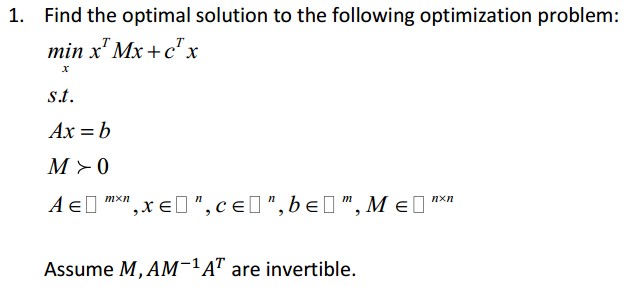
\includegraphics[width=0.7\textwidth]{pics/Task1_1}
\end{figure}

\subsection{Question 2}
\begin{figure}[h]
\centering
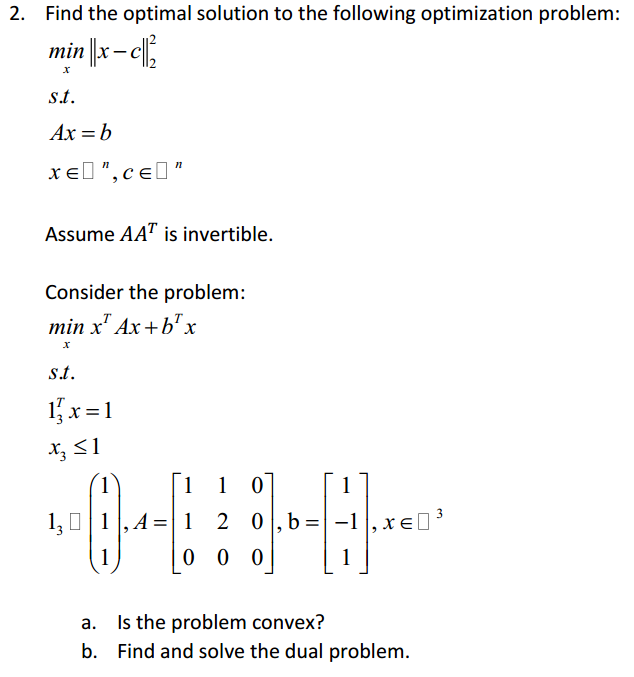
\includegraphics[width=0.7\textwidth]{pics/Task1_2}
\end{figure}

\subsection{Question 3}
\begin{figure}[h]
\centering
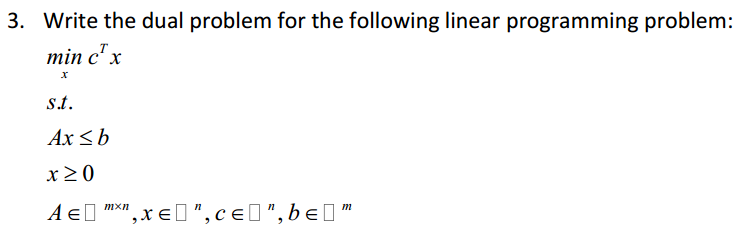
\includegraphics[width=0.7\textwidth]{pics/Task1_3}
\end{figure}

\section{Task 2}

\end{document}
